\documentclass{article}
\usepackage{../../settings}

\begin{document}
\hexcover{Py 心寫程式}{學習歷程}{作者:曾嘉禾}{Dandelion}{電算社}

\begin{large}
\begin{boxpar}{Dandelion}{說明}
透過 Python 的 pygame 函式庫寫出一款圖形化介面的遊戲。
\end{boxpar}
\begin{boxpar}{Dandelion}{動機}
    \begin{itemize}
\item 受到同校內學長姐啟發
\item 希望可以發揮自己寫程式的功力與其他人一起完成一款遊戲
\item 未來想當程式設計師
    \end {itemize}
\end{boxpar}
\begin{boxpar}{Dandelion}{遊戲內容}
    \begin{boxpar}{Dandelion}{第一關:躲避隕石}
        \begin{itemize}
            \item 玩家以滑鼠操控角色
            \item 躲避四面而來的隕石以取得勝利
        \end{itemize}
    \end{boxpar}
    \begin{boxpar}{Dandelion}{第二關:躲避隕石-鍵盤}
   \begin{itemize}
        \item 玩家以鍵盤左右操控角色
        \item 躲避由上而下的隕石以取得勝利
        \item 隕石以重力加速度向下
   \end{itemize}
    \end{boxpar}
    \begin{boxpar}{Dandelion}{第三關:打淑麗}
   \begin{itemize}
        \item 以校長為題材的遊戲
        \item 如同打殭屍一般的點擊正確按鈕以「打淑麗」
        \item 若按錯將延遲一段時間
   \end{itemize}
    \end{boxpar}
 \end{boxpar}

    \begin{boxpar}{Dandelion}{學習過程}
\begin{itemize}
    \item 問題:猶豫遊戲引擎的選擇
        \begin{itemize}
            \item 解決方法:仔細比較兩個遊戲引擎之間的差別
            \item 得到啟發:比較並且分析是在開始攻克目標之前的重要環節
        \end{itemize}
        \item 問題:惱人的 pygame.display
        \begin{itemize}
            \item 解決方法:上網查詢
            \item 得到啟發:鍛鍊程式設計師必要的技能—查詢以及閱讀能力
            \item 查詢的網站
                \begin{itemize}
                    \item Youtube:
                    \begin{itemize}
                        \item \url{https://www.youtube.com/watch?v=C8YtdC8mxTU}
                    \end{itemize}
                    \item Pygame 官網:
                        \begin{itemize}
                            \item \url{https://www.pygame.org/docs/ref/display.html}
                        \end{itemize}
                \end{itemize}
        \end{itemize}
\end{itemize}
    \end{boxpar}
\newpage
\begin{boxpar}{Dandelion}{成品}
    程式碼:\url{https://github.com/hsnucrc46/crcproject}\\
    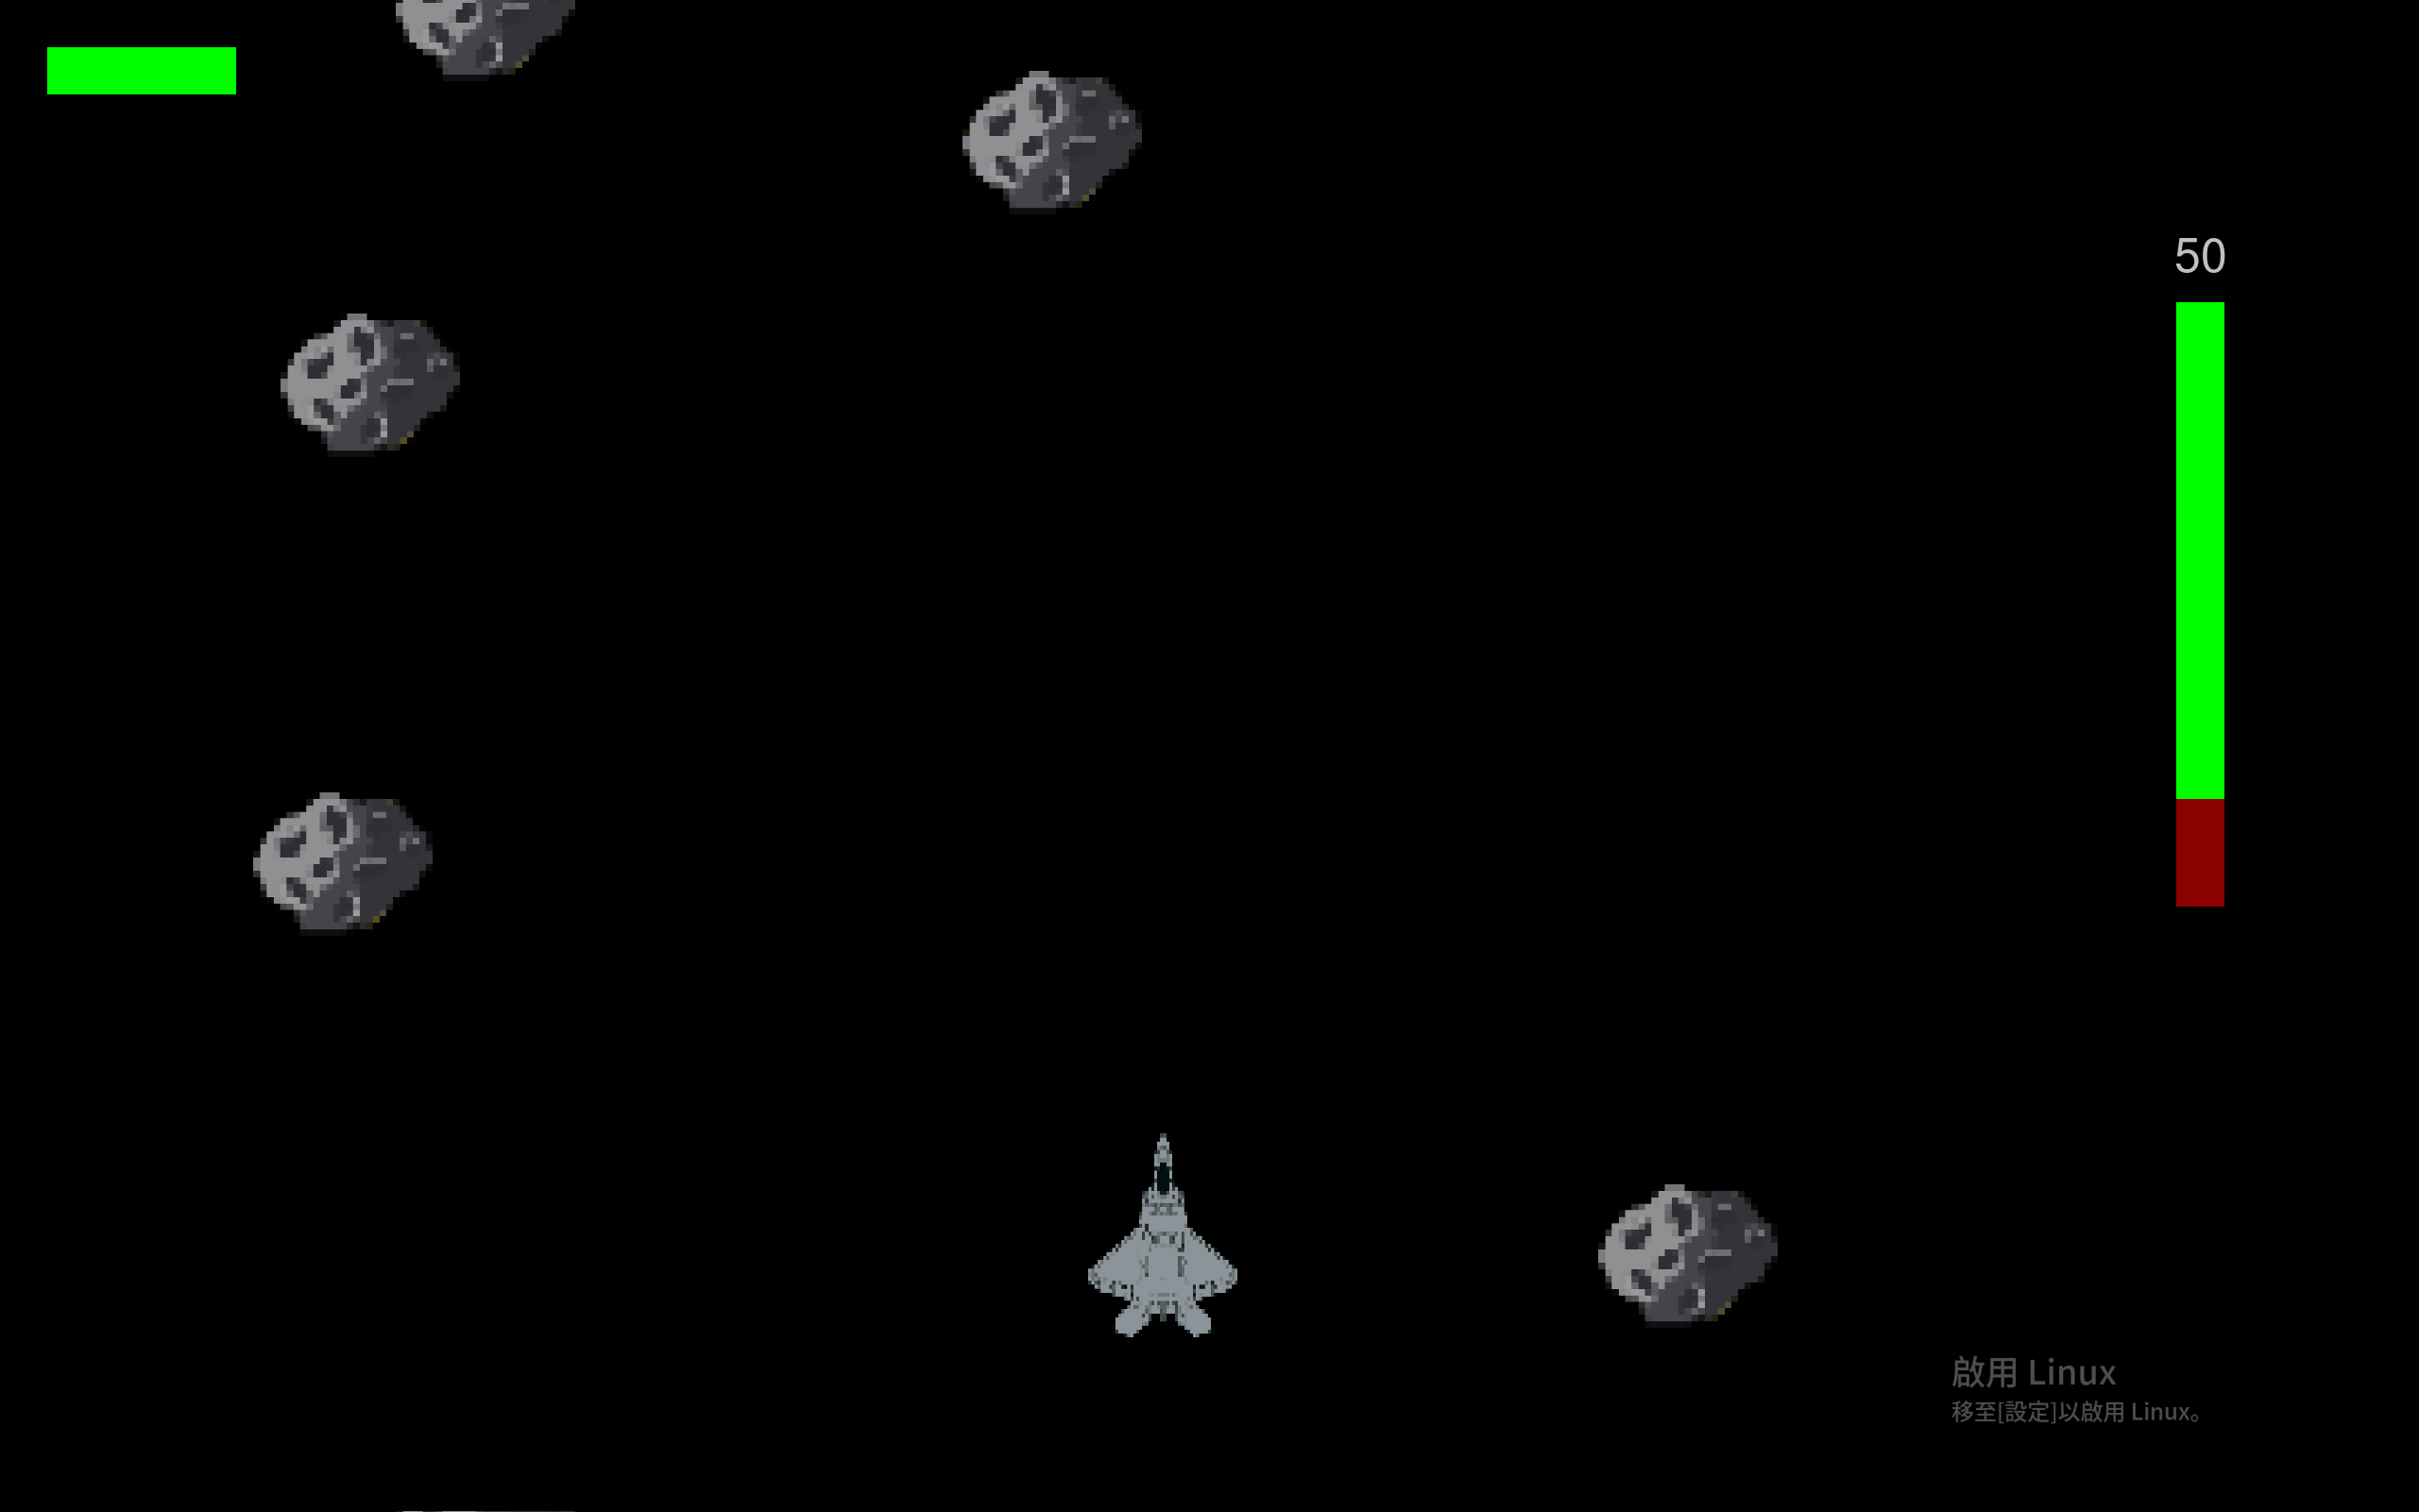
\includegraphics[width=\linewidth]{src/game.png}
\end{boxpar}
\end{large}
\end{document}
